\chapter{PLANTEAMIENTO DEL PROBLEMA}
\section{Descripción de la Realidad Problemática}

Las discapacidades del habla abarcan una amplia gama de condiciones que afectan la capacidad de una persona para comunicarse verbalmente de manera clara y fluida. Según la American Speech-Language-Hearing Association (ASHA), las discapacidades del habla pueden originarse por una variedad de razones, que van desde dificultades físicas en los órganos responsables de la producción del habla, hasta trastornos neurológicos que impactan la habilidad de hablar de manera clara y fluida.

Para las personas con discapacidades del habla, el lenguaje de señas se convierte en una herramienta invaluable que les permite expresar sus pensamientos, emociones y necesidades de manera efectiva. El lenguaje de señas es un sistema de comunicación visual y gestual utilizado por personas sordas o con discapacidades auditivas para comunicarse entre sí y con personas que pueden escuchar.

La Organización Mundial de la Salud afirmó que aproximadamente 70 millones de personas en el mundo son sordomudas. Un total de 360 millones de personas son sordas, y 32 millones de ellas son niños. Sin embargo, en Perú, de acuerdo con los resultados del Censo de Población y Vivienda 2017, como se puede observar en la Figura \ref{1:fig 1}, hay un elevado porcentaje de personas que tienen dificultades para oír y para hablar o comunicarse.

\begin{figure}[h]
	\begin{center}
		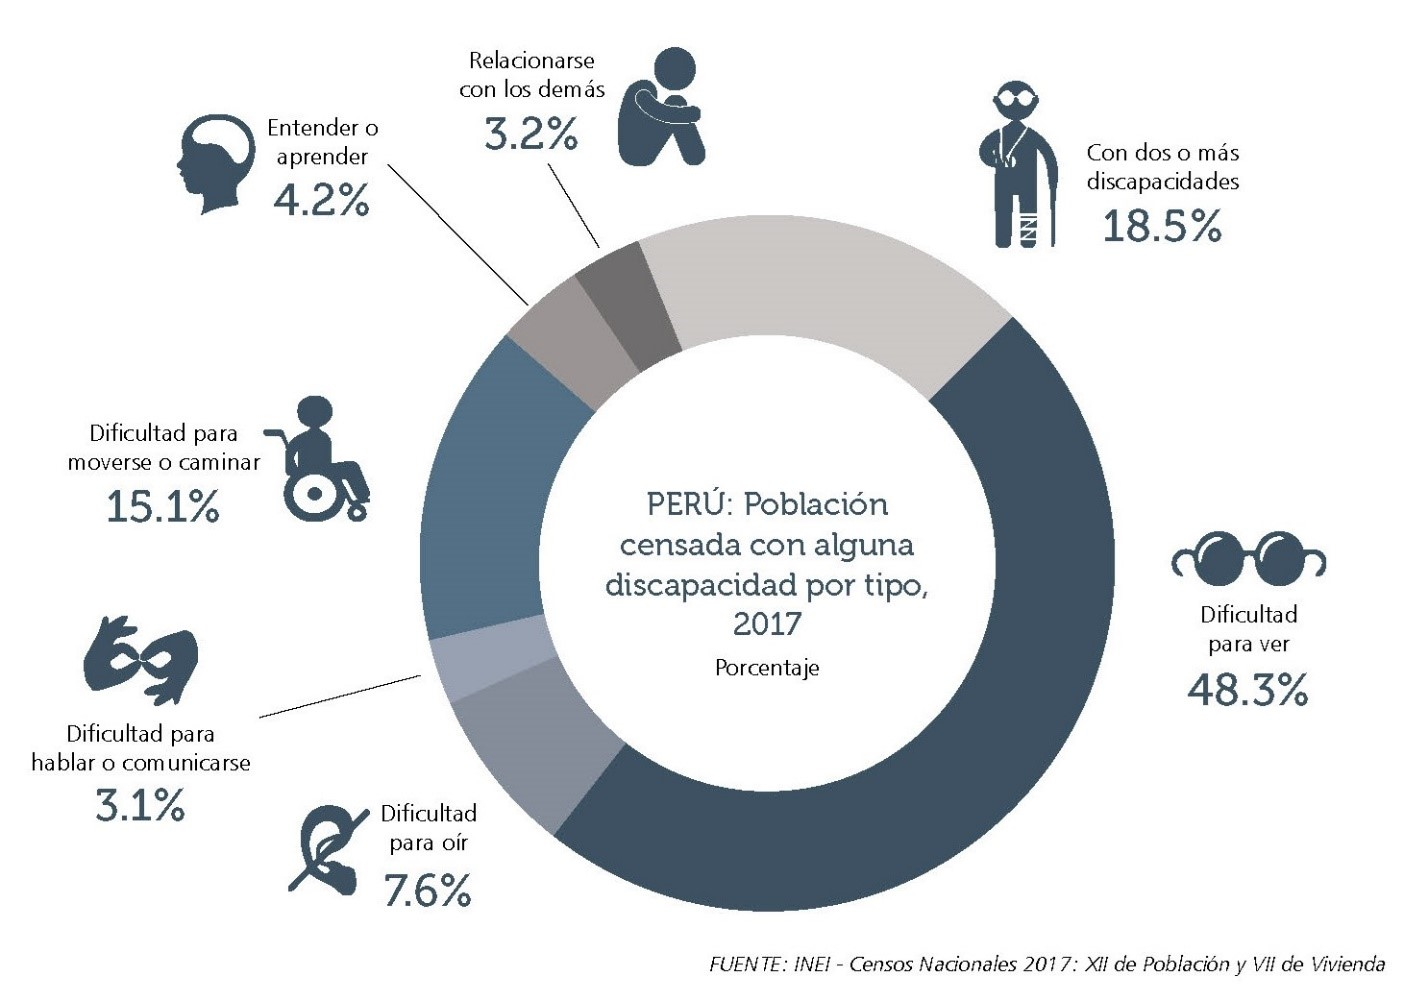
\includegraphics[width=0.5\textwidth]{1/figures/personas_discapacidad.jpg}
		\caption{\% de personas con discapacidad. Fuente: \cite{porcentaje de_personas_discapacidad}}
		\label{1:fig 1}
	\end{center}
\end{figure}

El INEI también afirma que las personas presentan estas capacidades utilizan como apoyo para comunicarse su voz (19,8\%), gesto y manos (11,9\%) y lenguaje de señas (2,9\%). Y debido a estas dificultades, estas personas se ven afectadas en el ámbito social y también laboral, por no poder expresarse debido a sus discapacidades. Según la Organización Mundial de Salud, las personas con estas discapacidades tienen más probabilidades de experimentar pobreza y exclusión social, y tienen menos probabilidades de tener un empleo remunerado que las personas sin discapacidades. En base a encuestas realizadas por la organización Incluyeme, alrededor del 72\% de personas con discapacidad se encuentra desempleado, como se puede observar en la Figura \ref{1:fig 2}.

\begin{figure}[h]
	\begin{center}
		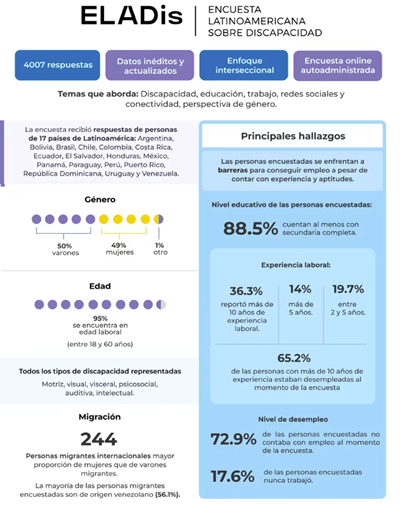
\includegraphics[width=0.25\textwidth]{1/figures/Encuesta_personas_discapacidad.png}
		\caption{Encuesta de personas con discapacidad . Fuente: \cite{encuesta_personas_discapacidad}}
		\label{1:fig 2}
	\end{center}
\end{figure}

El Deep Learning puede cambiar la forma de comunicación de las personas con discapacidades para comunicarse con personas sin ellas. Al entrenar modelos de Deep Learning con conjuntos de datos que contengan gestos de lenguaje de señas, es posible desarrollar modelos que puedan reconocer y traducir los gestos en tiempo real a texto. Estos modelos pueden capturar la complejidad de los movimientos de manos, dedos y expresiones faciales que son parte integral del lenguaje de señas. Además, al utilizar redes neuronales, estos modelos pueden aprender representaciones complejas de los gestos y expresiones, lo que les permite diferenciar dialectos de lenguaje de señas. 

El objetivo principal de esta investigación es lograr un aumento significativo en la comunicación entre personas con discapacidades del habla y aquellas que no las tienen, a través de la implementación de un modelo de traducción de lenguaje de señas utilizando Deep Learning. Este modelo busca facilitar una interacción más fluida y efectiva, permitiendo a las personas con discapacidades del habla expresar sus pensamientos, emociones y necesidades de manera más accesible y comprensible para quienes no conocen el lenguaje de señas.

\section{Formulación del Problema}


\subsection{Problema General}
\newcommand{\ProblemaGeneral}{
	¿De qué manera el uso de un modelo Deep Learning podría facilitar la comunicación para personas con discapacidades del habla para interactuar con personas que no conocen el lenguaje de señas?
}
\ProblemaGeneral
\subsection{Problemas Espec\'{i}ficos}
\newcommand{\Pbone}{
	¿De qué manera la falta de conjuntos de datos de lenguaje de señas de cada idioma afectar al modelo Deep Learning? 
}
\newcommand{\Pbtwo}{
	¿De qué manera el modelo Deep Learning pueden diferenciar entre los distintos tipos de lenguajes de señas?
}
\newcommand{\Pbthree}{
	¿Qué métricas son las más adecuadas para la precisión y rendimiento de un modelo de traducción de lenguaje de señas? 
}

\newcommand{\Pbfour}{
	¿Cuáles son las técnicas más adecuadas para el preprocesamiento y normalización de la base de datos de lenguaje de señas? 
}


\begin{itemize}
	\item \Pbone
	\item \Pbtwo
	\item \Pbthree
	\item \Pbfour
\end{itemize}

\section{Objetivos de la Investigación}
\subsection{Objetivo General}
\newcommand{\ObjetivoGeneral}{
Desarrollar un modelo Deep Learning que se utilizará como medio para la traducción de lenguaje de señas, permitiendo la comunicación entre personas con discapacidades del habla y personas sin conocimiento del lenguaje de señas.
}
\ObjetivoGeneral
\subsection{Objetivos Espec\'{i}ficos}
\newcommand{\Objone}{
Evaluar y comparar diferentes enfoques en los aumentos de datos para mejorar la representación de los conjuntos de datos de lenguaje de señas.
}
\newcommand{\Objtwo}{
Utilizar técnicas de aprendizaje automático para mejorar la precisión del modelo en la diferenciación entre los distintos tipos de lenguajes de señas. 
}
\newcommand{\Objthree}{
Evaluar diferentes métricas de evaluación de modelos Deep Learning, como Accuracy, Recall, F1-Score para la determinación del modelo más adecuado para la traducción adecuada de lenguaje de señas.
}
\newcommand{\Objtfour}{
	Realizar comparaciones entre diferentes técnicas de preprocesamiento y normalización de datos de lenguaje de señas, como normalización de iluminación, corrección de gestos ambiguos.
}

\begin{itemize}
	\item {\Objone}
	\item {\Objtwo}
	\item {\Objthree}
	\item {\Objtfour}
\end{itemize}

\section{Justificación de la Investigación}

\subsection{Teórica}
Esta investigación se realiza para determinar si se puede utilizar un modelo de Deep Learning para poder mejorar la comunicación de las personas con discapacidades del habla con personas sin conocimiento de lenguaje de señas. Esta solución tiene el potencial de mejorar la calidad de vida de este grupo de personas facilitando su comunicación de manera más efectiva y fluida.

\subsection{Práctica}
Al culminar la investigación, las personas con discapacidades podrán utilizar el modelo de traducción de lenguaje de señas basado en Deep Learning para mejorar de manera significativa la comunicación con las personas sin conocimiento del lenguaje de señas. Este modelo tiene el potencial de ofrecer una solución efectiva y tecnológicamente avanzada para mejorar la accesibilidad y la calidad de vida de este grupo de personas.

\subsection{Metodológica}. 
El desarrollo de un modelo de traducción de lenguaje de señas basado en Deep Learning ayudará a que se mejore la calidad de vida de las personas con discapacidades del habla, debido a que permitirá una comunicación más fácil con aquellos que no conocen el lenguaje de señas. Este modelo facilitará la interacción en diversos entornos, como en el trabajo, la educación y la vida diaria. Además, al ser una solución tecnológica, se espera que tenga un impacto positivo en la comunidad de personas con discapacidad del habla en general.

\section{Delimitación del Estudio}

\subsection{Espacial}
El estudio se realizará a nivel de la ciudad de Lima, enfocándose en videos de traductores de lenguaje de señas del Perú, que han brindado acceso a videos para el entrenamiento del modelo. 

\subsection{Temporal}
El período de desarrollo de la investigación será de nueve meses comenzando en abril de 2024 con la recopilación de información para la definición de la problemática y temas con el mismo fin.

\subsection{Conceptual}
La presente investigación se centrará en el desarrollo de un modelo de traducción de lenguaje de señas basado en Deep Learning para el idioma de señas peruano, con el objetivo de mejorar la comunicación y la accesibilidad de las personas con discapacidades del habla. Se limitará a la recopilación y análisis de datos relacionados con el lenguaje de señas peruano y las técnicas de Deep Learning, excluyendo otros lenguajes de señas y enfoques de traducción de lenguaje de señas

\section{Hipótesis}

\subsection{Hipótesis General}
\newcommand{\HipotesisGeneral}{
Mediante el desarrollo de un modelo de traducción de lenguaje de señas basado en Deep Learning se logrará mejorar la comunicación para personas con discapacidades del habla con personas que no conocen el lenguaje de señas, mejorando así su accesibilidad y calidad de vida.
}
\HipotesisGeneral
\subsection{Hipótesis Específicas}
\newcommand{\Hone}{
	Mediante el uso diferentes enfoques de técnicas de aumento de datos, sea posible mejorar la representación de los conjuntos de datos disponibles y compensar en parte la falta de datos específicos para el español peruano, lo que resultará en un mejor rendimiento del modelo de traducción de lenguaje de señas.
}
\newcommand{\Htwo}{
	El modelo Deep Learning aumentará su precisión significativa con lo que respecta de lenguaje de señas, lo que demuestra la eficacia de las técnicas de aprendizaje profundo en este contexto.
}
\newcommand{\Hthree}{
	La implementación de métricas de evaluación en los modelos Deep Learning aumentará las diferencias significativas entre los diferentes modelos evaluados, lo que permitirá la identificación del modelo más adecuado para la traducción de lenguaje de señas.
}
\newcommand{\Hfour}{
	La implementación de técnicas de preprocesamiento, mejoren la calidad de los datos de lenguaje de señas y con ello aumentar el rendimiento del modelo Deep Learning para la traducción de lenguaje de señas.
}

\begin{itemize}
	\item \Hone
	\item \Htwo
	\item \Hthree
	\item \Hfour
\end{itemize}

\subsection{Matriz de Consistencia}
A continuación se presenta la matriz de consistencia elaborada para la presente investigación (véase Anexo \ref{1:table}).

